\section{Linear Regression Baseline}
\label{sec:linreg}

This section establishes two classical baselines: ordinary least squares (OLS) regression
and GARCH(1,1). Both are transparent and well-understood, making their failure modes
informative for motivating the neural network architectures that follow.

\subsection{Standard Linear Regression}

\subsubsection{Setup}

An OLS model is trained on the 10 signed lag features with a standard train/test split.
Features and target are scaled with a \texttt{StandardScaler} fitted on the training set
only. The target $y_t = |r_t|$ is the realized absolute return, used throughout as a
proxy for next-day volatility. The model takes the form
\[
  \hat{y}_t = \beta_0 + \sum_{k=1}^{10} \beta_k \, r_{t-k}.
\]

\subsubsection{Results}

\begin{table}[H]
  \centering
  \caption{Linear regression performance on the test set (scaled units).}
  \label{tab:linreg_full}
  \begin{tabular}{lrrrr}
    \toprule
    Model & MAE & RMSE & QLIKE \\
    \midrule
    Linear Regression (raw lags)     & 0.638 & 0.933 & 16.79 \\
    Linear Regression (engineered)   & 0.598 & 0.874 &  7.46 \\
    \bottomrule
  \end{tabular}
\end{table}

\subsubsection{Coefficient Analysis}

\begin{table}[H]
  \centering
  \caption{OLS regression coefficients ranked by absolute magnitude.}
  \label{tab:coefficients}
  \begin{tabular}{lrr}
    \toprule
    Feature & Coefficient & $|\beta_k|$ rank \\
    \midrule
    lag\_9  & $-0.180$ & 1 \\
    lag\_8  & $-0.164$ & 2 \\
    lag\_10 & $-0.159$ & 3 \\
    lag\_7  & $-0.158$ & 4 \\
    lag\_5  & $-0.123$ & 5 \\
    lag\_6  & $-0.110$ & 6 \\
    lag\_3  & $-0.106$ & 7 \\
    lag\_1  & $-0.094$ & 8 \\
    lag\_4  & $-0.084$ & 9 \\
    lag\_2  & $-0.060$ & 10 \\
    \bottomrule
  \end{tabular}
\end{table}

All coefficients are \emph{negative} and small. This reveals the first fundamental
limitation:

\begin{quote}
  \textbf{Symmetry blindness.} Linear regression on signed returns cannot treat $+x$ and
  $-x$ identically. Predicting volatility requires $f(x) \approx f(-x)$ (the
  absolute value function), which a linear model cannot represent. The model ``gives up''
  by assigning small negative coefficients and predicting near-zero values for all inputs.
\end{quote}

\subsubsection{Predicted vs.\ Actual}

\begin{figure}[H]
  \centering
  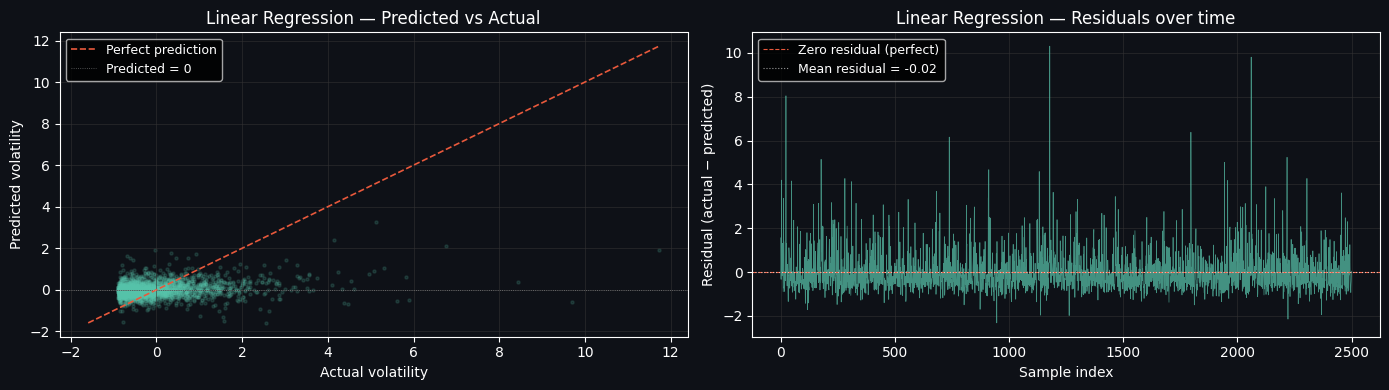
\includegraphics[width=\textwidth]{figures/figure_31.png}
  \caption{Linear regression: predicted vs.\ actual realized absolute return.
    The model systematically underpredicts during crisis episodes.}
  \label{fig:linreg_pred}
\end{figure}

The model produces a near-constant prediction close to zero throughout the entire sample.
Residuals are always positive and are dramatically amplified during crisis episodes.

\subsection{Feature Engineering}

Squaring the lag features forces the symmetry the model cannot learn from signed returns:
$r_{t-k}^2 = |r_{t-k}|^2$ treats positive and negative shocks of equal magnitude
identically. A \emph{recency ratio} feature $\nicefrac{r_{t-1}}{\text{mean}(r_{t-2:t-5})}$
is also added to capture short-term momentum in volatility.

\begin{table}[H]
  \centering
  \caption{Impact of feature engineering on linear regression performance.}
  \label{tab:feat_eng}
  \begin{tabular}{lrrrr}
    \toprule
    Features & MAE & RMSE & QLIKE \\
    \midrule
    Raw signed lags             & 0.638 & 0.933 & 16.79 \\
    Squared lags + recency ratio & 0.598 & 0.874 &  7.46 \\
    \midrule
    Improvement ($\Delta$)       & $+$6.3\% & $+$6.4\% & $+$55.6\% \\
    \bottomrule
  \end{tabular}
\end{table}

The QLIKE loss drops by 56\%, showing that manual feature engineering substantially
reduces systematic under-prediction. This foreshadows what the FNN can learn
\emph{automatically} from raw lags.

\subsection{Regime Analysis}

\begin{table}[H]
  \centering
  \caption{Linear regression performance by market regime (raw lag features).}
  \label{tab:linreg_regime}
  \begin{tabular}{lrrr}
    \toprule
    Regime  & MAE   & RMSE  & QLIKE \\
    \midrule
    Full    & 0.638 & 0.933 & 16.79 \\
    Calm    & 0.488 & 0.587 & 15.49 \\
    Crisis  & 1.987 & 2.367 & 28.46 \\
    \midrule
    Crisis / Calm ratio & $4.1\times$ & $4.0\times$ & $1.8\times$ \\
    \bottomrule
  \end{tabular}
\end{table}

During crisis periods, MAE is \textbf{4$\times$ higher} than during calm periods. The
model systematically underpredicts every volatility spike because it has no mechanism
to detect a regime shift. This is the second structural limitation:

\begin{quote}
  \textbf{Regime blindness.} A single linear model fitted on the full sample cannot
  adapt its behaviour to different market conditions.
\end{quote}

\subsection{GARCH(1,1) Baseline}

The GARCH(1,1) model provides a parametric volatility
benchmark. The conditional variance follows:
\[
  \sigma_t^2 = \omega + \alpha \, \epsilon_{t-1}^2 + \beta \, \sigma_{t-1}^2,
\]
where $\epsilon_t = r_t / \sigma_t$ are standardised residuals.

\subsubsection{Estimated Parameters}

\begin{table}[H]
  \centering
  \caption{GARCH(1,1) maximum-likelihood parameter estimates.}
  \label{tab:garch_params}
  \begin{tabular}{lrl}
    \toprule
    Parameter & Estimate & Interpretation \\
    \midrule
    $\omega$ (baseline variance) & 0.0159 & Long-run variance floor \\
    $\alpha$ (shock sensitivity) & 0.094  & Reaction to new shocks \\
    $\beta$  (persistence)       & 0.895  & Memory of past variance \\
    \midrule
    $\alpha + \beta$ (total persistence) & 0.989 & Near unit-root variance process \\
    Half-life of shock decay             & 60 days & Volatility shocks dissipate slowly \\
    \bottomrule
  \end{tabular}
\end{table}

The near-unit-root persistence ($\alpha + \beta = 0.989$) confirms that volatility
shocks take approximately \textbf{60 days} to decay to half their peak level.

\subsubsection{Regime Performance}

\begin{table}[H]
  \centering
  \caption{GARCH(1,1) performance by market regime (unscaled returns).}
  \label{tab:garch_regime}
  \begin{tabular}{lrrr}
    \toprule
    Regime  & MAE      & RMSE     & QLIKE    \\
    \midrule
    Full    & 0.00583  & 0.000069$^\dagger$ & $-$3.98 \\
    Calm    & 0.00506  & 0.000043$^\dagger$ & $-$4.17 \\
    Crisis  & 0.01281  & 0.000296$^\dagger$ & $-$2.27 \\
    \midrule
    Crisis / Calm ratio & $2.5\times$ & $6.9\times$ & --- \\
    \bottomrule
  \end{tabular}
  \par\smallskip
  \small $^\dagger$ These are MSE values; RMSE$= \sqrt{\text{MSE}}$.
\end{table}

GARCH improves on linear regression during calm periods but exhibits the same pattern
of regime degradation: crisis MAE is 2.5$\times$ higher than calm MAE. Despite its
elegant theoretical motivation, GARCH suffers from the third structural limitation:

\begin{quote}
  \textbf{Fixed functional form.} GARCH assumes a specific parametric update rule for
  variance. It cannot detect structural breaks or non-linear regime transitions.
\end{quote}

\subsection{Summary of Limitations}

\begin{table}[H]
  \centering
  \caption{Comparison of linear baseline models (MAE, full sample).}
  \label{tab:linreg_summary}
  \begin{tabular}{lcc}
    \toprule
    Model & MAE (full) & MAE (crisis) \\
    \midrule
    Linear Regression (raw lags)    & 0.638 & 1.987 \\
    Linear Regression (engineered)  & 0.598 & ---   \\
    GARCH(1,1)                      & 0.00583 & 0.01281 \\
    \bottomrule
  \end{tabular}
\end{table}

Three structural limitations motivate the turn to neural networks:

\begin{enumerate}
  \item \textbf{Symmetry blindness} (linear regression on signed inputs cannot represent
        $|x|$).
  \item \textbf{Regime blindness} (no model adapts its behaviour during crises).
  \item \textbf{Fixed functional form} (GARCH assumes a pre-specified update rule).
\end{enumerate}

A feedforward neural network with non-linear activations directly addresses limitation~1,
and deeper architectures are expected to partially address limitations~2 and~3.
